\documentclass[10pt,a4paper]{exam}
\usepackage[latin1]{inputenc}
\usepackage{amsmath}
\usepackage{amsfonts}
\usepackage{amssymb}
\usepackage{graphicx}
\usepackage{titlesec}
\usepackage{hyperref}
\usepackage{fancyeq}
\usepackage{tikz}
%\usepackage{tikz-uml}
\usepackage{mathpartir}
\usetikzlibrary{shapes,arrows,backgrounds,positioning}

\tikzset{
  treenode/.style = {align=center, inner sep=0pt, text centered,
    font=\sffamily},
  arn_n/.style = {treenode, circle, black, font=\sffamily\bfseries, draw=black,
    fill=white, text width=1.5em},% arbre rouge noir, noeud noir
  arn_r/.style = {treenode, circle, red, draw=red, 
    text width=1.5em, very thick},% arbre rouge noir, noeud rouge
  arn_x/.style = {treenode, rectangle, draw=black,
    minimum width=0.5em, minimum height=0.5em}% arbre rouge noir, nil
}

\usepackage[sc]{mathpazo}
\linespread{1.05}         % Palatino needs more leading (space between lines)
\usepackage[T1]{fontenc}

% some format settings
% for hard-bound final submission, use:
%\setlength{\oddsidemargin}{4.6mm}     % 30 mm left margin - 1 in
% for soft-bound version and techreport, use instead:
\setlength{\oddsidemargin}{-0.4mm}    % 25 mm left margin - 1 in
\setlength{\evensidemargin}{\oddsidemargin}
\setlength{\topmargin}{-5.4mm}        % 20 mm top margin - 1 in
\setlength{\textwidth}{160mm}         % 20/25 mm right margin
\setlength{\textheight}{237mm}        % 20 mm bottom margin
\setlength{\headheight}{5mm}
\setlength{\headsep}{5mm}
\setlength{\parindent}{0mm}
\setlength{\parskip}{\medskipamount}
\renewcommand\baselinestretch{1.2} % thesis format (not needed for techreport)
% don't let large figures hijack entire pages
\renewcommand\topfraction{.9}
\renewcommand\textfraction{.1}
\renewcommand\floatpagefraction{.8}

\pagestyle{headandfoot}
%\pointsinrightmargin
%\pointname{ marks}
%\marginpointname{ marks}

\marksnotpoints 

\hypersetup{  
  urlcolor=black,
  linkcolor=black,
  colorlinks=true  
}

\titlelabel{\llap{\thetitle\quad}}

\newcommand {\lbrac} {\makebox[0pt]{[\kern-1ex[}}
\newcommand {\rbrac} {\makebox[0pt]{]\kern-1ex]}}
\newcommand{\denote}[1]{\lbrac~#1~\rbrac}

\begin{document}

\begin{center}
\Large Algorithms \\
\LARGE \textbf{Exercise 6: Data structures IV \& Graph algorithms I} \\
\end{center}

\hrule

\vspace{0.5cm}

%\begin{center}
%\emph{Complete SECTION 1 and ONE other section.}
%\end{center}

\marksnotpoints
\pointsdroppedatright
\marksnotpoints
\marginpointname{ \points}

\begin{questions}

\section{Past Tripos questions}

\question[5] Given the following Fibonacci heap, where nodes with an asterisk are ``marked'', perform $\mathit{extractMin}()$ on it and then $\mathit{decreaseKey()}$ on the node whose key is currently 66, bringing it down to 4. Redraw the changed heap as you go along.

You need only draw any significant intermediate states of the heap, adding any necessary explanations so that a reader can follow what you are doing and why. \droppoints 
\begin{center}
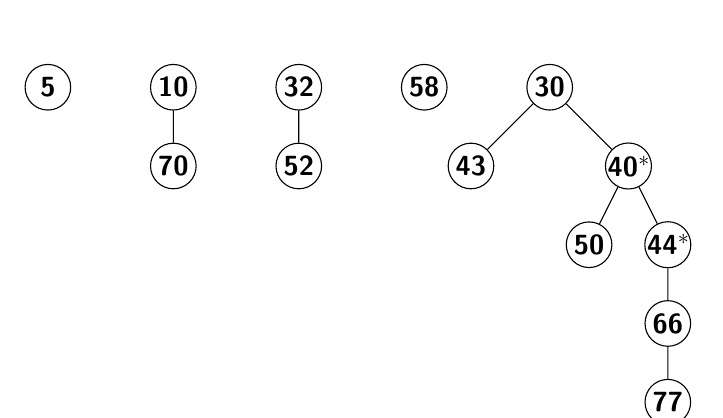
\begin{tikzpicture}[-,>=stealth',level/.style={sibling distance = 2cm/#1,
  level distance = 1.0cm}] 
  \node [arn_n](A) {5};
  \node [arn_n, right=of A](B) {10}
  	child { node[arn_n] {70}};
\node [arn_n, right=of B](C) {32}
	child { node[arn_n] {52}};
\node [arn_n, right=of C](D) {58};
\node [arn_n, right=of D](E){30}
    child{ node [arn_n] {43}  }
    child{ node [arn_n] {40$^{*}$}
            child{ node [arn_n] {50} 
            }
            child{ node [arn_n] {44$^*$}
							child{ node [arn_n] {66} child { node[arn_n] {77}}}
            }
		}
; 
\end{tikzpicture}
\end{center}

\question[5] Fibonacci heaps are designed so that their trees never become excessively ``wide and shallow''. Why? Justify this design goal in detail and then explain how it is achieved. \droppoints 

\question[10] Nothing, however, stops the trees in a Fibonacci heap from growing ``tall and narrow''. Prove this by describing a sequence of Fibonacci heap operations that, given an integer $n$, produces a Fibonacci heap made of a single tree consisting of a linear chain of $n$ nodes (in other words, each node in the tree except for the last one is the parent of exactly one node, and each node except for the first one is the child of exactly one node). \droppoints 

\section{Sorting functions}

\question[4] In programming languages with full type inference, such as ML or Haskell, we wish to infer the type for each function in a program. In order to do this, functions need to be sorted first: we cannot infer the type of a function
\begin{displaymath}
\mathbf{fun}~\mathit{bar}~x = \mathit{plus}~(\mathit{foo}~x)~(\mathit{foo}~x)
\end{displaymath}
unless we know what the types of $\mathit{plus}$ and $\mathit{foo}$ are first. We won't worry about the details of inferring types of functions here, but instead we will focus on sorting the functions based on their dependencies. Suppose that you are given the following types for a small functional programming language\footnote{Which is actually the syntax of the pure $\lambda$-calculus. Feel free to complete this exercise in a language of your choice -- the ML definitions are for reference only}:

\begin{displaymath}
\begin{array}{lcl}
\mathbf{datatype}~\mathit{expr} & = & \mathit{FUN}~\mathbf{of}~\mathit{string} \times \mathit{expr} \\
                                & \mid & \mathit{VAR}~\mathbf{of}~\mathit{string} \\
                                & \mid & \mathit{APP}~\mathbf{of}~\mathit{expr} \times \mathit{expr} \\\\
\mathbf{type}~\mathit{decl} & = & \mathit{string} \times \mathit{expr} \\
\mathbf{type}~\mathit{program} & = & \mathit{decl}~\mathit{list}
\end{array}
\end{displaymath}
An expression is either a single-parameter function (the $\mathit{FUN}$ constructor) which \emph{binds} a variable in a sub-expression, a variable (the $\mathit{VAR}$ constructor), or the application of one expression to another ($\mathit{APP}$). Declarations are named expressions and a program is a list of declarations.

Define a function $\mathit{fvs} : \mathit{expr} \to \mathit{string}~\mathit{list}$ which returns the list of \emph{free variables} in an expression. A variable is free if it is not bound by a function. Below are some examples of what $\mathit{fvs}$ should return:
\begin{displaymath}
\begin{array}{lcl}
\mathit{fvs}(\mathit{VAR}(\mathtt{"x"})) & = & \hslist{\mathtt{"x"}} \\
\mathit{fvs}(\mathit{FUN}(\mathtt{"x"}, \mathit{VAR}(\mathtt{"x"}))) & = & \hslist{} \\
\mathit{fvs}(\mathit{FUN}(\mathtt{"x"}, \mathit{VAR}(\mathtt{"y"}))) & = & \hslist{\mathtt{"y"}} \\
\mathit{fvs}(\mathit{APP}(\mathit{FUN}(\mathtt{"x"}, \mathit{VAR}(\mathtt{"x"})), \mathit{VAR}(\mathtt{"x"})) & = & \hslist{\mathtt{"x"}} 
\end{array}
\end{displaymath}
In the first example, $x$ is free because it is not bound by a function. In the second example, there is a function which binds $x$. In the third example, the function binds $x$, but $y$ is free. The last example is the most interesting because there are actually two variables named $x$. One is bound by the function in the left side of the $\mathit{APP}$ constructor. The second $x$ on the right, however, is free. \droppoints 
\question[4] Define a function $\mathit{dependencies} : \mathit{program} \to (\mathit{string} \times \mathit{string}~\mathit{list})~\mathit{list}$ which associates each declaration in a program with a list of its free variables. For example:
\begin{displaymath}
\begin{array}{cl}
 & \mathit{dependencies}([(\mathtt{"ID"}, \mathit{FUN}(\mathtt{"x"}, \mathit{VAR}(\mathtt{"x"}))), (\mathtt{"FOO"}, \mathit{FUN}(\mathtt{"x"}, \mathit{VAR}(\mathtt{"ID"})))]) \\
 = & \hslist{(\mathtt{"ID"}, \hslist{}), (\mathtt{"FOO"}, \hslist{\mathtt{"ID"}})}
\end{array}
\end{displaymath}
 \droppoints 
\question[6] Explain how topological sort could be used to sort the declarations in a program by their dependencies. In other words, given a value of type $(\mathit{string} \times \mathit{string}~\mathit{list})~\mathit{list}$ returned by $\mathit{dependencies}$, how would you sort it so that each declaration only depends on declarations which have appeared earlier on in the list? What happens if two or more declarations are mutually dependant on each other? \droppoints 
\question[10] A graph is said to be \emph{strongly connected} if every vertex is reachable from every other vertex. The \emph{strongly connected components} of an arbitrary directed graph are subgraphs that are themselves strongly connected. Below is a description of \emph{Kosaraju's algorithm} for finding the strongly connected components of a graph:
\begin{itemize}
\item Let $G$ be a directed graph and $S$ be an empty stack.
\item While $S$ does not contain all vertices:
\begin{itemize}
\item Choose an arbitrary vertex $v$ not in $S$. Perform a depth-first search starting at $v$. Each time that depth-first search finishes expanding a vertex $u$, push $u$ onto $S$.
\end{itemize}
\item Reverse the direction of all arcs to obtain the transposed graph.
\item While $S$ is non-empty:
\begin{itemize}
\item Pop the top vertex $v$ from $S$. Perform a depth-first search starting at $v$ in the transpose graph. The set of visited vertices will give the strongly connected component containing $v$; record this and remove all these vertices from the graph $G$ and stack $S$. 
\end{itemize}
\end{itemize}
Using a suitable value of type $\mathit{program}$, explain how this algorithm can be used to sort all the declarations within a program into groups of mutually dependant declarations. How does this compare to topological sort? \droppoints 
\question[10] (CSTs only) Implement Kosaraju's algorithm in a language of your choice. \droppoints 

\end{questions}
\end{document}